\section{Hybrid Quantum - Classical System} \label{Sec: Hybrid Quantum - Classical System}

This section reviews the structure and underpinning mathematics of hybrid quantum - classical algorithms, eg. VQAs.
Such techniques that involves both quantum and classical components have been proposed to address the limitation of NISQ devices \cite{brooksQuantumSupremacyHunt2019}.
Those restrictions include the lack of fault-tolerance design, the number of the available qubits per processors, and the depth of executable quantum circuits the practical use cases.

In more details, the hybrid techniques such as VQA allows development of \emph{parameterised circuits}, which act as a template and capable of receiving trainable parameters.
Those parameters can be used to sample circuits result iteratively in a quantum processor, and consequently be refined by a classical computer \cite{cerezo2021variational}.
In this way, we can rely on a wide range of classical optimisers to find the optimal circuit for a particular problem, as these optimisers only treat the variational circutis as black boxes capable of yielding outputs from inputs and the trainable parameters.



The process of solving a problem using VQAs involves three components: the \textit{training data}, the \textit{ansatzes}, and the \textit{Cost function}.
Consider a problem requires VQA to solve and given the training data, we can first construct a \textit{cost function} $C$.
By minimising the cost function value, we can obtain the optimal sequence of parameters $\theta$.
The variational circuit, called \textit{ansatz}, is the target of our training.
We aim to train the ansatz to so that its cost function $C(\theta)$ reaches the minimum value:
\begin{equation}
    \theta^* = \underset{\theta}{\arg \min} \;C(\theta)
    \label{Eqn: optimize theta with ansatz}
\end{equation}
The cost function $C(\theta)$ is estimated by a quantum computer, while we can select a wide range of classical optimiser to train the parameters $\theta$.
Figure \ref{Fig: VQA diagram} this hybrid architecture and demonstrate the training process in more detail.

% Consider a simple problem that we want to solve using VQA, given access to the training data.
% The first step is to construct a \textit{cost function} $C$ used to search for an optimal set of circuit parameters, which is achieved by minimising the cost function during the training process.
% We can simplify the development of variational circuits by composing the circuit templates called \textit{ansatze}.
% \textit{Ansatz} is the parameterised circuit that depends on a set of parameters $\theta$.
% We aim to train the ansatze by optimising the parameters $\theta$s so that the cost function $C$ reaches its minimum, thus satisfying:
% \begin{equation}
%     \theta^* = \underset{\theta}{\arg \min} \;C(\theta)
%     \label{Eqn: optimize theta with ansatz}
% \end{equation}

% In short, the cost function $C(\theta)$ is calculated using the quantum computer, while the classical optimiser trains the parameters $\theta$. Figure \ref{Fig: VQA diagram} explains the VQA architecture and elaborates its training process in more detail.
\todo{paraphrase}
\begin{figure}
    \centering
    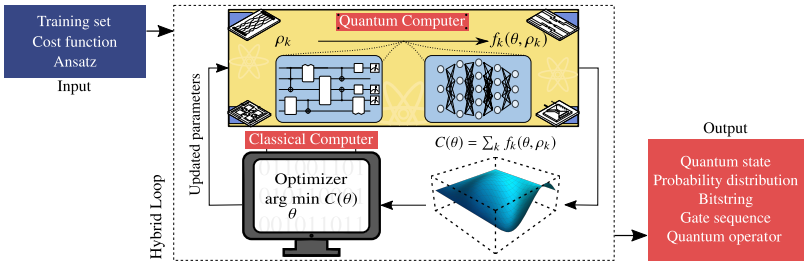
\includegraphics[width=\linewidth]{Appendices/vqadiagram.png}
    \caption{
        An illustrative diagram of a ganeral Variational Quantum Algorithm.
        The algorithm is a hybrid quantum-classical that involves:
        (1) A cost function $C(\theta)$;
        (2) An ansatz that receives trainable parameter $\theta$ and yields outputs from inputs;
        (3) A set of training data $\{\rho_k\}$ so the ansatz can learn the pattern.
        We use the quantum computer to calculate the cost function $C(\theta)$ for each step of optimisation.
        An optimisation algorithm in a classical computer is in charge to find the global minima in the cost landscape of $C(\theta)$, thus satisfy Eq. (\ref{Eqn: optimize theta with ansatz}).
        VQA's result is an approximation of the problem solution, which can be probability distribution, bit string, gate sequence and quantum operator.
        Figure from Cerezo et al. \cite{cerezo2021variational}.
    }
    \label{Fig: VQA diagram}
\end{figure}




\subsection{The Cost Function} \label{Sec: The Cost Function}\

% Encoding the problem into a cost function is the first step in solving a problem using VQA \cite{cerezo2021variational}.
% The cost function is equivalent to that used in classical machine learning.
% It maps the values of the trainable parameters $\theta$ into real values, which represent the measure of distance from an optimum solution.
% For a function $f$ that receives input states $\{\rho_k\}$, observables $\{O_k\}$, and a parameterized circuit $U(\theta)$, the cost is expressed as:

Both classical machine learning and quantum machine learning use the cost function to map the the trainable parameters $\theta$ into a value that represent the distance from the optimal solution.
This is the first step in finding a solution using VQA \cite{cerezo2021variational}.
For a function $f$ with the input states $\{\rho_k\}$, the observables $\{O_k\}$ and the parameterised circuit $U(\theta)$, the cost is as following equation:

\begin{equation}
    C(\theta) = f(\{\rho_k\}, \{O_k\}, U(\theta)) \;,
\end{equation}
or this equation with a set of functions $\{f_k\}$ and the trace $Tr$ as the square of a distance matrix:
\begin{equation}
    C(\theta) = \sum_k f_k \left(\Tr[ O_k U(\theta) \rho_k U^\dagger(\theta) ]\right) \;,
    \label{Eqn: Cost function}
\end{equation}

A cost function of an VQA algorithm must meet a number of criteria:
(1) The cost function must be 'faithful' and 'operationally meaningful', the minimum value of $C(\theta)$ should correspond to the optimal solution of the problem, and we can expect the better solution with lower cost function value in general;
(2) The cost function must be 'efficiently estimated' on a quantum computer by measuring qubits values;
(3) The cost function must be 'trainable', such that the parameters $\theta$ could be efficiently optimised.
\subsection{Ansatze} \label{Sec: Ansatze}
\begin{figure}
    \centerline{
    \Qcircuit @C=1em @R=0em {
    & \multigate{2}{U_1(\theta_1)}    & \multigate{2}{U_2(\theta_2)}    & \qw &        & & \multigate{2}{U_L(\theta_L)}   & \qw\\
    & \ghost{U_1(\theta_1)}           & \ghost{U_2(\theta_2)}           & \qw & \cdots & & \ghost{U_L(\theta_L)}          & \qw\\
    & \ghost{U_1(\theta_1)}           & \ghost{U_2(\theta_2)}           & \qw &        & & \ghost{U_L(\theta_L)}          & \qw
    \gategroup{1}{2}{3}{7}{.6em}{--}
    }
    }
    \centerline{$U(\theta)$}
    \centerline{}
    \centerline{}
    \centerline{
    \Qcircuit @C=1em @R=0em{
    & \multigate{1}{}   & \ctrl{2}  & \gate{}           & \qw \\
    & \ghost{}          & \qw       & \multigate{1}{}   & \qw \\
    & \gate{}           & \targ     & \ghost{}          & \qw
    \gategroup{1}{2}{3}{4}{.6em}{--}
    }
    }
    \centerline{$U_l(\theta_l)$}
    \caption{
        A diagram of a sample ansatz (above), the ansatz is a sequence of unitaries $U_l(\theta_l)$ (below).
        The unitary $U(\theta)$ receives parameters $\theta$ is expressed by $L$ layers of unitaries $U_l(\theta_l)$ for $l$ is the layer indices.
        Each $U_l(\theta_l)$ is a circuit composed of a mix of parameterised and unparametrised gates.
    }\label{Fig: Ansatz diagram}
\end{figure}

In physics and mathematics, \emph{ansatz} (plural \emph{ansatze}) is an educated guess or a starting point from which you start looking for a solution to the problem at hand. In quantum computing, \emph{ansatz} is a parameterised circuit, formed as a sequence of unitary (or "atomic") circuits, which is used as a framework for the circuit optimisation.
In general, the location of parameters $\theta$ is determined by the ansatz form and can be trained to minimise the cost.
The ansatz structure can be defined based on the problem (called 'problem-inspired ansatze') or a generic structure (called 'problem agnostic ansatze') that can be used without any relevant information available \cite{cerezo2021variational}.

The cost function in Eq. (\ref{Eqn: Cost function}) encodes the parameters $\theta$ in a unitary $U(\theta)$ and applies to the input states of the circuit.
The figure \ref{Fig: Ansatz diagram} shows that $U(\theta)$ can be expressed as a product of $L$ consecutive unitaries:
\begin{equation}
    U(\theta) = U_L(\theta_L) \cdots U_2(\theta_2) U_1(\theta_1)\;,
\end{equation}
with each layer:
\begin{equation}
    U_l(\theta_l) = \prod_m e^{-i\theta_m H_m} W_m
\end{equation}
for unparamaterized unitary $W_m$, hermitian operator $H_m$, and $\theta_l$ is the $l$-th element of $\theta$.
\subsection{Gradients} \label{Sec: Gradients}
After defining the cost function and a suitable ansatz, we train the parameter $\theta = \{\theta_{l}\}$ to solve the problem in Eq. (\ref{Eqn: optimize theta with ansatz}) \cite{cerezo2021variational}.
The cost function gradient helps the optimiser to find the global minima.
Consider the cost function in Eq. (\ref{Eqn: Cost function}), for a unitary that parameterises rotation $e^{i \theta_l \sigma_{l}}$, where $\theta_l$ be the $l$-th element of $\theta$, $\sigma_l$ is a Pauli rotation operator.
We can evaluate the gradient with the parameter-shift rule:
\begin{equation}
    \frac{\partial C}{\partial\theta_l}
    = \sum_k \frac{1}{2 \sin{\alpha}}
    \left(
    \Tr[O_k U^\dagger(\theta_+) \rho_k U(\theta_+)]
    - \Tr[O_k U^\dagger(\theta_-) \rho_k U(\theta_-)]
    \right) \;,
    \label{Eqn: Parameter-shift rules}
\end{equation}
with $\theta_{\pm} = \theta \pm \alpha e_l$, $\alpha \in \mathbb{R}$ and $e_l$ is a vector such that its $l$-th position have the value of 1, or else 0.

Essentially, we can shift the $l$-th parameter by some amount $\alpha$, and Eq. (\ref{Eqn: Parameter-shift rules}) will calculate the gradient.

\subsection{Optimisers} \label{Sec: Optimisers}
The accuracy of VQA greatly depends on the optimisation method.
Typically, we can achieve the solution by making successive moves along the gradient direction.
This optimisation approach is within the scope of stochastic gradient descent (SGD).
One example of SGD is the ADAM optimiser \cite{kingmaAdamMethodStochastic2014}, which can vary the size of the steps taken during optimisation to produce more efficient and precise results compared to the basic SGD.